\section{图上的函数}
\label{sec:graph-vertex-edge-functions}

在同一张图上，我们可以给每个测点记录一个温度，也可以给每条管道记录一个流量。前一类数值附着在顶点上，后一类数值附着在边上。固定顶点与边的编号顺序后，这两组数各自排成列向量，构成顶点空间与边空间；关联矩阵正是连接这两个空间的线性算子。本节先建立顶点函数与边流量向量的坐标表示，再定义关联矩阵并完整推导它的两种作用。

\subsection{顶点函数}
\label{sec:incidence-vertex-functions}

图~\ref{fig:incidence-running-example}画出了本章反复使用的四点五边图$\mathcal{G}=(V,E)$。四条外圈边围成一个四元环，另有一条对角边连接顶点$1$和$3$。顶点集和边集分别为
\[
V=\{1,2,3,4\},\qquad E=\{12,23,34,41,13\},
\]
其中$ij$简记连接顶点$i$与$j$的边。图中每个顶点旁标注了一个实数读数，依次为$3,2,1,0$。

给每个顶点赋一个实数，就得到图上的一个\term{顶点函数}（vertex function）$f\colon V\to\mathbb{R}$。图的顶点与边决定哪些位置直接相连，函数值则是在这一连接结构上附加的观测或状态数据。同一张图在不同应用场景中可以承载测点温度、地面海拔或节点电势——底层的图结构不变，改变的只是顶点上的函数值。

\begin{figure}[!htb]
  \centering
  \begingroup
\definecolor{IncidenceBlue}{HTML}{7188A3}
\definecolor{IncidenceInk}{HTML}{3B4252}
\begin{tikzpicture}[
  x=2.55cm,y=1.68cm,
  incidence vertex/.style={circle,draw=FigureStroke,fill=white,
    line width=.68pt,minimum size=5mm,inner sep=0pt,
    font=\footnotesize,text=IncidenceInk},
  incidence edge/.style={-{Stealth[length=2mm]},draw=FigureStroke,line width=.82pt},
  incidence reading/.style={text=IncidenceInk,font=\footnotesize,inner sep=3pt}
]
  \node[incidence vertex] (one) at (0,1) {$1$};
  \node[incidence vertex] (two) at (1,1) {$2$};
  \node[incidence vertex] (three) at (1,0) {$3$};
  \node[incidence vertex] (four) at (0,0) {$4$};
  \draw[incidence edge] (one) -- (two);
  \draw[incidence edge] (two) -- (three);
  \draw[incidence edge] (three) -- (four);
  \draw[incidence edge] (four) -- (one);
  \draw[incidence edge,draw=IncidenceBlue] (one) -- (three);
  \node[incidence reading,left=3mm of one] {$f(1)=3$};
  \node[incidence reading,right=3mm of two] {$f(2)=2$};
  \node[incidence reading,right=3mm of three] {$f(3)=1$};
  \node[incidence reading,left=3mm of four] {$f(4)=0$};
\end{tikzpicture}
\endgroup

  \caption{本章的四点五边图及一组顶点读数。黑灰色实线是四条外圈环边，蓝色实线是对角边$13$。边上的箭头给出记录沿边差分与边流量时使用的参考方向。顶点旁标注的读数排成列向量$\bm{f}=(3,2,1,0)^\top$。}
  \label{fig:incidence-running-example}
\end{figure}

对$n=|V|$个顶点固定一个排列次序$v_1,\ldots,v_n$，把各点上的函数值按此顺序排成列向量，顶点函数$f$就与$n$维列向量
\[
\bm{f}=\bigl(f(v_1),\ldots,f(v_n)\bigr)^\top\in\mathbb{R}^n
\]
一一对应。两个顶点函数可以逐顶点相加，也可以同乘一个实数，运算规则与$\mathbb{R}^n$中的向量加法和数乘完全一致。因此，图上全体实值顶点函数构成一个$n$维线性空间，记为$\mathbb{R}^V\cong\mathbb{R}^n$。对每个顶点$v\in V$，仅在顶点$v$处取$1$、在其余顶点处均取$0$的单位脉冲函数对应标准基向量$\bm{e}_v\in\mathbb{R}^V$，全部$n$个顶点的标准基向量$\{\bm{e}_{v_1},\ldots,\bm{e}_{v_n}\}$构成$\mathbb{R}^V$的一组标准正交基，任意顶点函数均可展开为$\bm{f}=\sum_{v\in V}f(v)\bm{e}_v$。

在顶点空间$\mathbb{R}^V$上，两个顶点函数$\bm{f},\bm{g}$的标准内积定义为各顶点读数乘积之和：
\begin{equation}
\langle\bm{f},\bm{g}\rangle_V=\bm{f}^\top\bm{g}=\sum_{v\in V}f(v)\,g(v).
\label{eq:incidence-vertex-inner-product}
\end{equation}
有限维线性空间中的基、坐标与内积可参考\BookChapterRef{chap:linear-representation}{卷二"线性空间"章}。

重新给顶点编号相当于对向量坐标施加一次置换。例如将顶点排列次序从$1,2,3,4$改为$3,1,4,2$，列向量的四个分量随之重排，但每个测点本身的读数并未改变。只要在计算前固定一套顶点编号次序，向量的每个分量就唯一对应一个顶点。本章固定按$1,2,3,4$排列图~\ref{fig:incidence-running-example}中的读数，得到
\[
\bm{f}=(3,2,1,0)^\top.
\]
这组顶点读数将在后续计算中反复使用。

\subsection{边函数}
\label{sec:incidence-edge-functions}

与给每个顶点赋值的顶点函数相对应，给每条边赋一个实数就得到图上的一个\term{边函数}（edge function）$q\colon E\to\mathbb{R}$。对$m=|E|$条边固定一个编号次序$e_1,\ldots,e_m$，边函数$q$便与$m$维列向量
\[
\bm{q}=\bigl(q(e_1),\ldots,q(e_m)\bigr)^\top\in\mathbb{R}^m
\]
一一对应，全体实值边函数构成$m$维线性空间$\mathbb{R}^E\cong\mathbb{R}^m$。在图~\ref{fig:incidence-running-example}的四点五边图上，$m=5$；本章固定边的排列顺序为$12,23,34,41,13$，每个边函数写成五维列向量$\bm{q}=(q_{12},q_{23},q_{34},q_{41},q_{13})^\top\in\mathbb{R}^5$。

与顶点上的标量读数不同，沿边传递的量（如流量、电流或电位差）带有方向性。为了用实数坐标无歧义地记录方向，我们为每条无向边$e=\{u,v\}$预先指定一个箭头方向$u\to v$作为\emph{参考方向}（reference orientation），称$u$为该参考方向下的尾端（tail）、$v$为头端（head）。在图~\ref{fig:incidence-running-example}中，五条边的参考方向依次约定为$1\to2$、$2\to3$、$3\to4$、$4\to1$和$1\to3$。

当边函数用于记录沿边输送的有向数量时，在给定参考方向下，边空间中的向量$\bm{q}\in\mathbb{R}^E$称为图上的一个\term{边流量}（edge flow，也称边流量向量），其第$e$个分量$q_e\in\mathbb{R}$表示边$e$上的有向流量：
\begin{itemize}
\item 若$q_e>0$，表示边$e$上的实际流向与参考方向$u\to v$一致，流量大小为$q_e$；
\item 若$q_e<0$，表示边$e$上的实际流向与参考方向相反（即沿$v\to u$流动），流量大小为$|q_e|$；
\item 若$q_e=0$，表示边$e$上没有流量。
\end{itemize}
例如在边$41$（参考方向为$4\to1$）上，若记录$q_{41}=-2$，实际含义是从顶点$1$流向顶点$4$的流量为$2$个单位。对无向图而言，参考方向只是一种坐标记账约定：同一股实际物理流如果改用相反的参考方向记录，其坐标分量$q_e$变号，但实际流向与流量大小丝毫不变。

在后续章节中，我们需要严格区分边流量$q_e$与边权$w_e$这两类边上数据。边流量$\bm{q}\in\mathbb{R}^E$是随外部输入或状态变化的变量，反转边$e$的参考方向会使坐标$q_e$变号；而边权$w_e\geq 0$是图本身的结构参数（如管道容导、支路电导或连接强度），反转参考方向不会改变非负边权$w_e$的数值。后续将$m$条边的权重排成$m\times m$对角矩阵$\bm{C}=\operatorname{diag}(w_{e_1},\ldots,w_{e_m})$。

在边空间$\mathbb{R}^E$上，两个边向量$\bm{q},\bm{r}\in\mathbb{R}^E$的标准内积定义为对应边分量乘积之和：
\begin{equation}
\langle\bm{q},\bm{r}\rangle_E=\bm{q}^\top\bm{r}=\sum_{e\in E}q_e\,r_e.
\label{eq:incidence-edge-inner-product}
\end{equation}
本章讨论环空间与割空间的正交分解时始终使用这一标准内积。到第~\ref{chap:graph-electrical-networks}章研究电网络时，为了按支路电阻计量电功率耗散，还会引入以电阻矩阵加权的边内积；不同内积定义了不同的正交关系，使用时须加以区分。

\subsection{关联矩阵的作用}
\label{sec:incidence-matrix-actions}

建立了顶点空间$\mathbb{R}^V$和边空间$\mathbb{R}^E$之后，我们用一张矩阵把这两个空间连接起来。

给定有$n$个顶点、$m$条边的图$\mathcal{G}=(V,E)$并固定各边的参考方向。对每一条有向参考边$e\colon u\to v$，我们在矩阵的第$e$列中，于尾端$u$所在的行填$+1$，于头端$v$所在的行填$-1$，其余各行均填$0$。这样构造出的$n\times m$矩阵$\bm{B}\in\mathbb{R}^{n\times m}$称为图$\mathcal{G}$的\term{关联矩阵}（incidence matrix，更确切地称为带符号关联矩阵），其第$e$列可写为顶点空间两个标准基向量之差：
\begin{equation}
\bm{B}_{:,e}=\bm{e}_u-\bm{e}_v,\qquad e\colon u\to v.
\label{eq:incidence-oriented-column}
\end{equation}
由于无自环图的每条边连接两个不同端点，$\bm{B}$的每一列恰好含有一个$+1$和一个$-1$，其余$n-2$个元素全为$0$，因此每一列的元素之和恒等于零。

按顶点顺序$1,2,3,4$排矩阵的行，按边顺序$12,23,34,41,13$（参考方向依次为$1\to2,2\to3,3\to4,4\to1,1\to3$）排矩阵的列，图~\ref{fig:incidence-running-example}中四点五边图的关联矩阵为
\[
\bm{B}=
\begin{pmatrix}
 1 & 0 & 0 & -1 & 1\\
 -1 & 1 & 0 & 0 & 0\\
 0 & -1 & 1 & 0 & -1\\
 0 & 0 & -1 & 1 & 0
\end{pmatrix}.
\]
以第四列（对应边$41\colon 4\to1$）为例：尾端是顶点$4$，所以第$4$行填$+1$；头端是顶点$1$，所以第$1$行填$-1$；顶点$2$和$3$不是边$41$的端点，第$2,3$行均填$0$。

关联矩阵$\bm{B}$及其转置$\bm{B}^\top$分别诱导了方向相反的两个基本线性映射：$\bm{B}^\top\colon\mathbb{R}^V\to\mathbb{R}^E$把顶点函数映射为边空间中的向量，$\bm{B}\colon\mathbb{R}^E\to\mathbb{R}^V$把边流量向量映射回顶点空间。下面依次考察这两个映射的具体含义。

\paragraph{沿边取差}

先看转置矩阵$\bm{B}^\top\in\mathbb{R}^{m\times n}$对顶点函数$\bm{f}\in\mathbb{R}^V$的作用。$\bm{B}^\top$的第$e$行正是$\bm{B}$的第$e$列转置$(\bm{e}_u-\bm{e}_v)^\top$。用这一行左乘列向量$\bm{f}$，得到的第$e$个分量恰好是边$e\colon u\to v$的尾端读数$f(u)$减去头端读数$f(v)$：
\[
(\bm{B}^\top\bm{f})_e=(\bm{e}_u-\bm{e}_v)^\top\bm{f}=f(u)-f(v).
\]
对全部$m$条边同时执行这一运算，就得到边空间中的一个$m$维列向量$\bm{d}=\bm{B}^\top\bm{f}\in\mathbb{R}^E$，其第$e$个分量为
\begin{equation}
d_e=(\bm{B}^\top\bm{f})_e=f(u)-f(v),\qquad e\colon u\to v.
\label{eq:incidence-edge-difference}
\end{equation}
我们把由顶点函数$\bm{f}$生成的边向量$\bm{d}=\bm{B}^\top\bm{f}\in\mathbb{R}^E$称为$\bm{f}$的\term{沿边差分}（edge difference，或沿边差分向量），而把线性算子$\bm{B}^\top\colon\mathbb{R}^V\to\mathbb{R}^E$称为沿边差分算子。需要明确的是：单个分量$d_e=f(u)-f(v)$是边$e$上的标量差值，而$\bm{B}^\top\bm{f}$则是将所有边上的差值按边序排列而成的$m$维边向量。

我们在四点五边图上对读数$\bm{f}=(3,2,1,0)^\top$逐边计算其沿边差分向量$\bm{B}^\top\bm{f}$：
\begin{itemize}
\item 边$12$（$1\to2$）：$d_{12}=f(1)-f(2)=3-2=1$；
\item 边$23$（$2\to3$）：$d_{23}=f(2)-f(3)=2-1=1$；
\item 边$34$（$3\to4$）：$d_{34}=f(3)-f(4)=1-0=1$；
\item 边$41$（$4\to1$）：$d_{41}=f(4)-f(1)=0-3=-3$；
\item 边$13$（$1\to3$）：$d_{13}=f(1)-f(3)=3-1=2$。
\end{itemize}
将五个分量按边序排成列向量，得到
\[
\bm{B}^\top\bm{f}=(1,1,1,-3,2)^\top\in\mathbb{R}^5.
\]

如果给每个顶点的读数同时加上同一个常数$c\in\mathbb{R}$，即把$\bm{f}$替换为$\bm{f}+c\bm{1}$，那么任意一条边$e\colon u\to v$上的差值变为
\[
\bigl(f(u)+c\bigr)-\bigl(f(v)+c\bigr)=f(u)-f(v),
\]
常数增量$c$在尾端与头端相减时完全抵消。特别地，若顶点函数在所有顶点上取同一个常数$c$（即常值向量$\bm{f}=c\bm{1}$），则它的沿边差分向量为零向量$\bm{B}^\top(c\bm{1})=\bm{0}$——各点读数毫无差别，沿边自然没有变化。

\paragraph{按顶点汇总}

再看关联矩阵本身$\bm{B}\colon\mathbb{R}^E\to\mathbb{R}^V$对边流量向量$\bm{q}\in\mathbb{R}^E$的作用。按行读取$\bm{B}$：在第$v$行中，所有以顶点$v$为尾端（从$v$出发）的边系数为$+1$，所有以顶点$v$为头端（进入$v$）的边系数为$-1$，不以$v$为端点的边系数为$0$。因此，用$\bm{B}$的第$v$行左乘边流量向量$\bm{q}$，就是把从顶点$v$流出的总流量减去流入顶点$v$的总流量，所得结果称为顶点$v$处的\term{净流出量}（net outflow）：
\begin{equation}
(\bm{B}\bm{q})_v=\sum_{e:\,v\text{ 是尾端}}q_e
              -\sum_{e:\,v\text{ 是头端}}q_e.
\label{eq:incidence-net-outflow}
\end{equation}
将全部$n$个顶点的净流出量排成列向量，就得到顶点空间中的\emph{净流出向量}$\bm{B}\bm{q}\in\mathbb{R}^V$。

以四点图中的顶点$1$为例。$\bm{B}$的第一行在边$12,41,13$处非零：边$12$（$1\to2$）和边$13$（$1\to3$）以顶点$1$为尾端，系数为$+1$；边$41$（$4\to1$）以顶点$1$为头端，系数为$-1$。因此顶点$1$的净流出量为
\[
(\bm{B}\bm{q})_1=q_{12}-q_{41}+q_{13}.
\]

为了看清单条边上的流量如何影响各个顶点，取只在第一条边$12$上携带$1$个单位正向流量的边流量向量$\bm{q}=\bm{e}_{12}=(1,0,0,0,0)^\top$。左乘$\bm{B}$恰好取出$\bm{B}$的第一列：
\[
\bm{B}(1,0,0,0,0)^\top=(1,-1,0,0)^\top.
\]
可以看到，尾端顶点$1$的净流出量为$+1$，头端顶点$2$的净流出量为$-1$（即净流入$1$），其余顶点$3,4$的净流出量均为$0$。

一般的边流量向量$\bm{q}=\sum_{e\in E}q_e\bm{e}_e$是各条边流量的叠加，对应的净流出向量为
\[
\bm{B}\bm{q}=\sum_{e\colon u\to v}q_e(\bm{e}_u-\bm{e}_v).
\]
在每一条边$e\colon u\to v$上，从尾端$u$流出的量$+q_e$必定等于进入头端$v$的量（记作净流出$-q_e$）。把所有$n$个顶点的净流出量相加，即用全一向量$\bm{1}^\top$左乘$\bm{B}\bm{q}$，每条边的$+q_e$与$-q_e$都成对抵消：
\[
\sum_{v\in V}(\bm{B}\bm{q})_v
=\bm{1}^\top(\bm{B}\bm{q})
=\sum_{e\colon u\to v}(q_e-q_e)=0.
\]
这说明：无论边流量向量$\bm{q}\in\mathbb{R}^E$取何值，全图所有顶点的净流出量总和恒为零。

图~\ref{fig:incidence-matrix-actions}把$\bm{B}^\top$与$\bm{B}$的两种基本计算放在同一条参考边$1\to2$上并排对照：左图由两端读数$f(1)=3,f(2)=2$相减得到该边上的沿边差分分量$d_{12}=1$；右图由该边上的单位流量$q_{12}=1$在尾端$1$记净流出$+1$、在头端$2$记净流出$-1$。

\begin{BookInlineFigure}
  \centering
  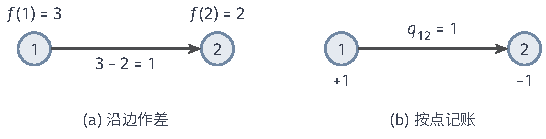
\includegraphics{figures/03-graphs/05-matrices-and-spectra/tikz/incidence-matrix-actions/figure.pdf}
  \caption{同一条参考边$1\to2$上的两种对偶运算。(a) 沿边差分算子$\bm{B}^\top$将两端顶点读数作差，得到边分量$d_{12}=f(1)-f(2)=1$。(b) 净流出汇总算子$\bm{B}$将该边上的单位正向流量$q_{12}=1$分配到两端，尾端净流出为$+1$，头端净流出为$-1$。}
  \label{fig:incidence-matrix-actions}
\end{BookInlineFigure}

\paragraph{伴随恒等式}

沿边差分算子$\bm{B}^\top\colon\mathbb{R}^V\to\mathbb{R}^E$与按顶点汇总算子$\bm{B}\colon\mathbb{R}^E\to\mathbb{R}^V$在矩阵形式上互为转置，在几何上则关于顶点内积与边内积互为伴随算子。

任取一个顶点函数$\bm{f}\in\mathbb{R}^V$和一个边流量向量$\bm{q}\in\mathbb{R}^E$。先算出沿边差分向量$\bm{B}^\top\bm{f}\in\mathbb{R}^E$，再与$\bm{q}$在边空间中作内积，按式~\eqref{eq:incidence-edge-inner-product}展开为对所有边的求和：
\[
\langle\bm{B}^\top\bm{f},\bm{q}\rangle_E
=\sum_{e\colon u\to v}\bigl(f(u)-f(v)\bigr)q_e
=\sum_{e\colon u\to v}\bigl(f(u)q_e-f(v)q_e\bigr).
\]
在最右端的求和式中，每条边$e\colon u\to v$产生了两项：尾端$u$处带有正号项$+f(u)q_e$，头端$v$处带有负号项$-f(v)q_e$。现在把求和次序从“逐边相加”改为“逐顶点归并”：固定一个顶点$w\in V$，把所有以$w$为尾端的边所贡献的$+f(w)q_e$与所有以$w$为头端的边所贡献的$-f(w)q_e$收集到一起，提出公因子$f(w)$，括号内剩下的恰好就是式~\eqref{eq:incidence-net-outflow}中顶点$w$的净流出量$(\bm{B}\bm{q})_w$：
\[
\begin{aligned}
\sum_{e\colon u\to v}\bigl(f(u)q_e-f(v)q_e\bigr)
&=\sum_{w\in V}f(w)\Biggl(\sum_{e:\,w\text{ 是尾端}}q_e-\sum_{e:\,w\text{ 是头端}}q_e\Biggr)\\
&=\sum_{w\in V}f(w)(\bm{B}\bm{q})_w.
\end{aligned}
\]
根据顶点内积定义式~\eqref{eq:incidence-vertex-inner-product}，最右端正是$\bm{f}$与净流出向量$\bm{B}\bm{q}$在顶点空间中的内积。于是我们得到伴随恒等式：
\begin{equation}
\langle\bm{B}^\top\bm{f},\bm{q}\rangle_E
=\langle\bm{f},\bm{B}\bm{q}\rangle_V.
\label{eq:incidence-adjoint-pairing}
\end{equation}
从代数上看，式~\eqref{eq:incidence-adjoint-pairing}就是向量内积的转置性质$(\bm{B}^\top\bm{f})^\top\bm{q}=\bm{f}^\top(\bm{B}\bm{q})$；从图上的记账来看，它表明“按每条边把两端读数差乘以边流量再求和”与“按每个顶点把读数乘以净流出量再求和”算的是同一笔总账。下一节证明环空间与割空间正交时，这一恒等式将起到核心作用。

最后说明参考方向的选择对计算结果的影响。如果将某一条边$e$的参考方向从$u\to v$反转为$v\to u$，矩阵$\bm{B}$的第$e$列随之变号；与此同时，同一股实际流量在新参考方向下的坐标$q_e$也变号。在计算$\bm{B}\bm{q}$时，列向量的负号与流量坐标的负号相乘抵消，因此每个顶点的净流出量$(\bm{B}\bm{q})_v$完全不变。

同理，沿边差分分量$(\bm{B}^\top\bm{f})_e$虽随参考方向变号，但与同样变号的$q_e$相乘后乘积不变。这意味着参考方向只是边空间坐标系的符号约定，顶点处的物理守恒关系以及下一节建立的子空间结构均不依赖于参考方向的具体选取。
